\begin{figure}
\centering
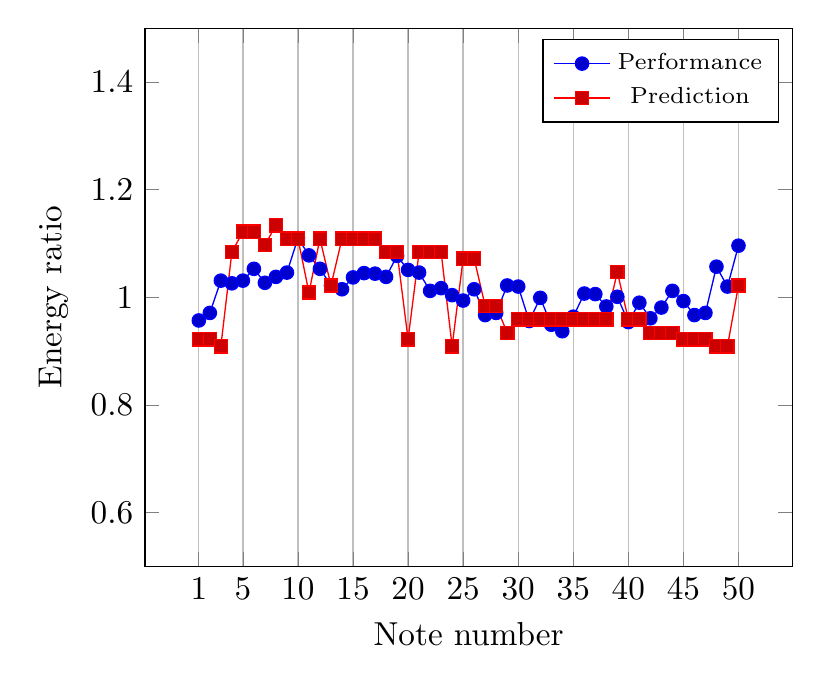
\begin{tikzpicture}[scale=1.2]

\begin{axis}[legend style={font=\scriptsize},
		ylabel={Energy ratio},
        xlabel={Note number},
        ymin=0.5, ymax=1.5,
        xtick={1,5,10,15,20,25,30,35,40,45,50},
        xmajorgrids]

    \addplot coordinates {(1,0.957) (2,0.971) (3,1.031) (4,1.026) (5,1.031) (6,1.053) (7,1.027) (8,1.038) (9,1.046) (10,1.11) (11,1.078) (12,1.053) (13,1.022) (14,1.015) (15,1.037) (16,1.045) (17,1.044) (18,1.038) (19,1.077) (20,1.051) (21,1.046) (22,1.012) (23,1.017) (24,1.004) (25,0.994) (26,1.015) (27,0.967) (28,0.971) (29,1.022) (30,1.02) (31,0.956) (32,0.999) (33,0.949) (34,0.937) (35,0.964) (36,1.007) (37,1.006) (38,0.983) (39,1.001) (40,0.954) (41,0.99) (42,0.961) (43,0.981) (44,1.012) (45,0.993) (46,0.967) (47,0.971) (48,1.057) (49,1.02) (50,1.096)};
  

    \addplot coordinates {(1,0.922) (2,0.922) (3,0.909) (4,1.084) (5,1.122) (6,1.122) (7,1.097) (8,1.134) (9,1.109) (10,1.109) (11,1.009) (12,1.109) (13,1.022) (14,1.109) (15,1.109) (16,1.109) (17,1.109) (18,1.084) (19,1.084) (20,0.922) (21,1.084) (22,1.084) (23,1.084) (24,0.909) (25,1.072) (26,1.072) (27,0.984) (28,0.984) (29,0.934) (30,0.959) (31,0.959) (32,0.959) (33,0.959) (34,0.959) (35,0.959) (36,0.959) (37,0.959) (38,0.959) (39,1.047) (40,0.959) (41,0.959) (42,0.934) (43,0.934) (44,0.934) (45,0.922) (46,0.922) (47,0.922) (48,0.909) (49,0.909) (50,1.022)};
    
     \addlegendentry{Performance}
    

   \addlegendentry{Prediction}

\end{axis}
\end{tikzpicture}

\caption[Energy Ratio in performance and prediction]{Energy Ratio in performance and prediction}
\label{fig:energy}
\end{figure}